\documentclass[a4paper, titlepage]{livret}													% classe spéciale rapport : livret

\usepackage[utf8]{inputenc} 																% accents
\usepackage[T1]{fontenc} 																	% caractères français
\usepackage{geometry} 																		% marges
\usepackage[francais]{babel}																% langue
\usepackage{graphicx} 																		% images
\usepackage{verbatim} 																		% texte préformaté
\usepackage{listings} 																		% code source
\usepackage{listingsutf8} 																	% code source accents
\usepackage[final]{pdfpages}																% inclusion de pdf
\usepackage{url} 																			% utilisation des url
\usepackage{caption} 																		% nom des tableaux
\usepackage{amsmath} 																		% maths
\usepackage{amsfonts} 																		% fonts maths
\usepackage{stmaryrd} 																		% intervalles d'entiers
\usepackage[lined,boxruled,french]{algorithm2e} 											% algorithmique
\usepackage[framed,numbered,autolinebreaks,useliterate]{mcode}								% code

\SetKwInput{Precondition}{Pré-condition(s)}	 												% macro algorithme préconditions
\SetKwInput{Declaration}{Déclaration(s)} 													% macro algorithme déclarations
\SetKw{KwDA}{en décroissant jusqu'à}	 													% macro algorithme downto
\def\siecle#1{\textsc{\romannumeral #1}\textsuperscript{e}~siècle} 							% macro pour l'écriture des siècles
\graphicspath{{img/}}																		% chemin des illustrations

\title{Projet d'Analyse Numérique}															% titre
\author{Elliot Sisteron & Antoni Markovski}													% auteur        

\pagestyle{headings}																		% rappel discret (en haut à gauche)

\begin{document}


\includepdf{pdf/cover.pdf}                													% page de garde

\setcounter{tocdepth}{2}
\tableofcontents																			% table des matières

\chapter*{Introduction}
\addcontentsline{toc}{chapter}{Introduction}												% ajouter l'introduction au sommaire
	En sciences appliquées, nous sommes souvent amenés à résoudre des systèmes d'équations.
	En effet, les chercheurs passent la plupart de leur temps à déduire des \og inconnues \fg{} à partir de données concrètes.
	C'est pourquoi il est primordial de pouvoir résoudre de tels systèmes de manière efficace (c'est-à-dire de déterminer des solutions exactes ou très bien approchées) et rapide (avec un nombre d'opérations relativement faible).

	Nous nous intéresserons dans ce projet à un cas bien particulier de résolution de systèmes d'équations linéaires : celui de Cholesky.
	En plus d'être une méthode dite \og directe \fg{} (c'est-à-dire permettant de déduire de manière exacte les solutions du système en un nombre fini d'opérations), nous verrons qu'elle a la particularité d'accélérer significativement les calculs.

	Nous présenterons d'abord rapidement les conditions nécessaires à l'application de cette méthode ainsi que son fonctionnement.
	Ensuite, nous nous intéresserons à l'implémentation de ce procédé en langage Fortran.
	Enfin, nous l'appliquerons à des données pour en tester l'efficacité, ce qui nous permettra alors de faire un bilan concernant la rapidité d'exécution de cette méthode.

\chapter{Présentation de la méthode de Cholesky}
	Pour résoudre un système d'équations linéaires, on se ramène souvent à son expression matricielle : 
		\[ Ax = b \]
		\[ A \in \mathcal{M}_{n,n} \quad x, b \in \mathcal{M}_{n,1} \]
	Si la matrice $A$ est pleine, on cherche souvent à se ramener à des cas plus simples pour résoudre le système.
	En l'occurence, le procédé de Cholesky est basé sur une méthode de factorisation de la matrice $A$ en deux matrices triangulaires plus faciles à traiter.
	Il s'agit d'un cas particulier de décomposition $LU$ avec $L \in \mathcal{LT}$ (triangulaire inférieure : $L$ower), et $U \in \mathcal{UT}$ (triangulaire supérieure : $U$pper).
	
	\section{De Gauss à Cholesky}
		\subsection{Pivot de Gauss}
			Johann Carl Friedrich Gauss est un mathématicien allemand ayant beaucoup contribué à l'avancement des mathématiques au \siecle{18}.
			Sa renommée fût telle qu'on le surnomma \og Le prince des mathématiciens \fg{}.
			Il utilisa à plusieurs reprises un algorithme aujourd'hui appellé \og Élimination de Gauss \fg{} ou \og Pivot de Gauss \fg{} lui permettant de résoudre des systèmes d'équations linéaires.
			Cette méthode était déjà connu des chinois depuis le \siecle{1} avant JC.

			Elle consiste à se ramener à un système triangulaire équivalent par transformations linéaires.
				\[Ax = b \Leftrightarrow A'x = b'\]
			avec $A' \in \mathcal{UT}$.
		
		\subsection{Factorisation LU et résolution par remontée}
			Cette factorisation peut être considérée comme l'interprétation matricielle de l'élimination de Gauss.
			On peut en déduire une factorisation de la matrice en deux matrices triangulaires par l'algorithme de Doolittle :
				\[A = LU \]
				\[ L \in \mathcal{LT} \quad U \in \mathcal{UT} \]
			$L$ étant à diagonale unité pour conserver l'unicité de la décomposition. On aurait pu par exemple avoir $U$ à diagonale unité (décomposition de Crout).
			Nous ne détaillerons pas ici son fonctionnement, toutefois il est important de noter les deux choses suivantes :
			\begin{enumerate}
				\item Son coût est de $\frac{2n^{2}}{3}$
				\item Une condition suffisante pour qu'une matrice $A \in \mathcal{M}_{n,n}$ soit factorisable est que toutes ses sous-matrices principales soient régulières (c'est-à-dire inversibles). Cette décomposition est unique du fait que $L$ ait une diagonale unité.
			\end{enumerate}

			Dès lors, il est facile de réécrire le système de la manière suivante :
				\[ LUx = b \] 
			En posant $Ux = y$, on en déduit :
				\[ Ly = b \]
			$L$ étant triangulaire inférieure à diagonale unité :
				\[ 
					L = 
					\begin{pmatrix}
						1 & 0 & \cdots & \cdots & 0\\
						l_{2,1} & 1 & 0 & \cdots& \vdots \\
						l_{3,1} & l_{3,2} & 1 & \cdots\\
						\vdots& \vdots & \vdots & \ddots & \vdots \\
						l_{n,1} & \cdots & \cdots & \cdots & 1\\
					\end{pmatrix} 
				\]
			On a :
				\begin{align*}
					Ly = b \
					\Leftrightarrow &
						\ \begin{pmatrix}
							1 & 0 & \cdots & \cdots & 0 \\
							l_{2,1} & 1 & 0 & \cdots & \vdots \\
							l_{3,1} & l_{3,2} & 1 & \cdots & \vdots\\
							\vdots& \vdots & \vdots & \ddots & \vdots \\
							l_{n,1} & \cdots & \cdots & \cdots & 1\\
						\end{pmatrix} .
						\begin{pmatrix}
							y_{1} \\
							y_{2} \\
							\vdots \\
							\vdots \\
							y_{n} \\
						\end{pmatrix} =
						\begin{pmatrix}
							b_{1} \\
							b_{2} \\
							\vdots \\
							\vdots \\
							b_{n} \\
						\end{pmatrix} \\
					\Leftrightarrow &
						\ \begin{pmatrix}
							y_{1} \\
							y_{1}l_{2, 1} + y_{2} \\
							\vdots \\
							\vdots \\
							\sum_{i = 1}^{n} y_{i}l_{n, i}\\
						\end{pmatrix} =
						\begin{pmatrix}
							b_{1} \\
							b_{2} \\
							\vdots \\
							\vdots \\
							b_{n} \\
						\end{pmatrix}
				\end{align*}
			Ce qui peut alors se résoudre par une méthode de descente, c'est-à-dire en remarquant que :
				\[y_{1} = b_{1}\]
			Puis que :
				\[\forall i \in \llbracket 1,n \rrbracket,\ y_{i} = b_{i} - \sum_{j = 1}^{i-1} y_{j}l_{i, j} \] 
			Enfin, il convient de résoudre le sytème :
				\[Ux = y\]
			$U$ étant triangulaire supérieure, on peut effectuer le même raisonnement que précédemment et résoudre le système par une méthode de remontée :
				\[x_{n} = \frac{y_{1}}{u_{n,n}}\]
				\[\forall i \in \llbracket 1,n \rrbracket,\ x_{i} = \frac{y_{i} - \sum_{j = i+1}^{n} x_{j}u_{i, j}}{u_{i,i}} \]

			\newpage
			Calculons le coût des algorithmes de descente et de remontée successifs.
			Basons-nous pour cela sur le procédé de remontée, à chaque calcul de $x_{i}$ il est demandé d'effectuer :
			\begin{itemize}
				\item $1$ division
				\item $(n - i)$ additions
				\item $(n - i)$ multiplications.
			\end{itemize}
			Le coût est donc :
				\[C = \sum_{i = 1}^{n} (1 + 2(n - i)) = n + 2(n^{2} - \frac{(n)(n + 1)}{2}) = n^{2}\]
			Ainsi, on en déduit que :
			\begin{itemize}
				\item L'algorithme de remontée requiert $n^{2}$ opérations
				\item L'algorithme de descente requiert $n^{2} - n$ opérations car il n'y a pas de divisions
				\item La succession de ces deux procédé demande donc $2n^{2} - n$ opérations.
			\end{itemize}
			La factorisation successive de Gauss puis de la descente/remontée a donc un coût de $\frac{2n^{3}}{3} + 2n^{2} - n$ opérations.

		\subsection{Décomposition $LL^{T}$ de Cholesky}
			André-Louis Cholesky était un mathématicien polytechnicien français de la fin du \siecle{19} - début du \siecle{20}. De nos jours, son nom est passé à la postérité grâce à la découverte de sa méthode de résolution de systèmes linéaires encore grandement utilisée aujourd'hui. Toutefois, il fut un temps où cette méthode n'était connue que de seconde main car Cholesky ne publiait pas ses découvertes. Sa famille a récemment déposé des papiers à l'école Polytechnique, dont un manuscrit exposant son procédé, formant ainsi le fonds A. Cholesky.
			Ce manuscrit écrit aux alentours de 1910, alors que Cholesky effectuait un temps légal de deux ans en tant que commandant de batterie, est un document scientifique de première importance.
			\begin{figure}[!ht]
				\centering
  					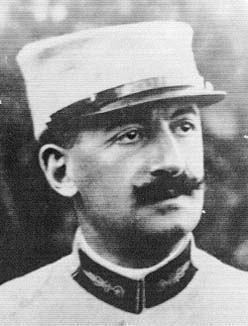
\includegraphics[scale=0.7]{cholesky.jpg}
  					\caption{André-Louis Cholesky}
			\end{figure}
			
			La méthode de Cholesky repose sur le principe, démontré en 1907 par Otto Toeplitz, que pour une matrice $A \in \mathcal{M}_{n,n}$ symétrique définie positive (ou hermitienne définie positive si l'on travaille avec des complexes) on peut effectuer une décompostion $LU$ bien particulière où $U = L^{T}$ (ou $U = L^{*}$ pour une matrice complexe) et réciproquement.
				
			Plus précisément, si $A$ est une matrice symétrique réelle (resp. complexe hermitienne) $\Leftrightarrow A = A^{T} \ (resp. \ A = A^{*})$ alors on a :
				\[
					\forall x \in \mathcal{M}_{n,1} \ / \ x \neq 0_{\mathcal{M}_{n,1}}, \ \langle Ax, x \rangle > 0 \\
					\Leftrightarrow
					\exists L \in \mathcal{LT} \ / \ A = LL^{T} \ (resp. \ A = LL^{*})
				\]

			À noter que la matrice $L$ est unique si on la choisit à diagonale strictement positive.
			On ne démontrera pas ici ce théorème de cours.
			Une question nous vient toutefois à l'esprit : comment vérifier que $A$ est définie positive ?
			
			En fait, si $A$ est symétrique (ou hermitienne), 
				\[ 
					\forall x \in \mathcal{M}_{n,1} \ / \ x \neq 0_{\mathcal{M}_{n,1}}, \ \langle Ax, x \rangle > 0
					\Leftrightarrow
					\forall k \in \llbracket 1,n \rrbracket, \ det(A_{k}) \neq 0
				\]
			Il s'agit du critère de Sylvester.

			Mais ce critère, comme pour la méthode $LU$, est très laborieux à vérifier. On cherche donc une condition suffisante simple pour qu'une matrice soit définie positive (il est déjà simple de vérifier qu'elle est symétrique).
			Si $A$ est symétrique réelle,
				\[ 
					\forall x \in \mathcal{M}_{n,1} \ / \ x \neq 0_{\mathcal{M}_{n,1}}, \ \langle Ax, x \rangle > 0
					\Leftrightarrow
					\forall \lambda_{i} \in \sigma(A) \ \lambda_{i} > 0
				\]
			avec $\sigma(A)$ le spectre de $A$ (c'est-à-dire l'ensemble des valeurs propres de $A$).
			Cela reste un critère relativement difficile à vérifier (il implique de devoir calculer toutes les valeurs propres de la matrice…).
			C'est pourquoi dans notre programme nous nous contenterons de vérifier simplement que la matrice $A$ est symétrique.
			On pourra toutefois s'arrêter lorsque l'on effectue une opération impossible dans la méthode de Cholesky (par exemple une racine sur un élément négatif ou bien une division par $0$) et signaler à l'utilisateur que cela signifie peut-être que la matrice rentrée n'est pas définie positive.

	\section{Exposé de la méthode de factorisation $LL^{T}$}
		Dans le manuscrit déposé par la famille d'André Cholesky se trouve l'explication de sa méthode de résolution des systèmes d'équations linéaires.

		\begin{figure}[!ht]
			\centering
  				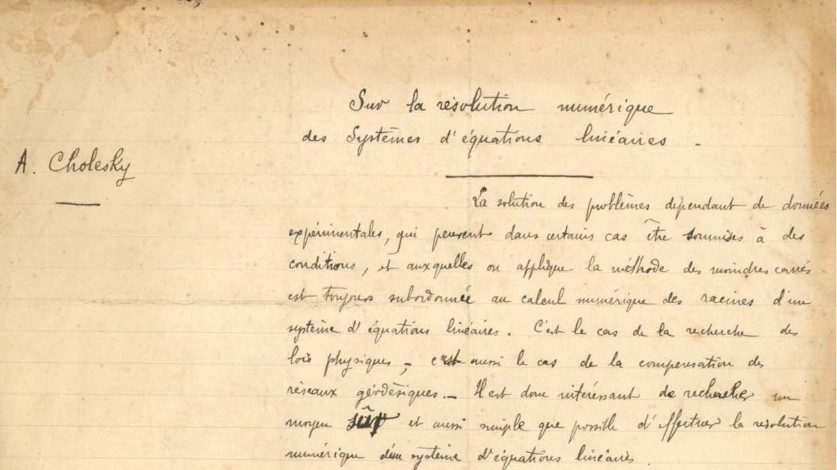
\includegraphics[scale=0.4]{manuscrit.jpg}
  				\caption{Un extrait du manuscrit écrit par Cholesky en 1910}
		\end{figure}
		
		Pour rappel, on dispose d'une matrice $A$ réelle symétrique (ou complexe hermitienne mais on ne détaillera pas ce cas) définie positive et l'on cherche à trouver une matrice $L \in \mathcal{LT}$ telle que $A = LL^{T}$.
		On peut donc écrire que :
			\[
				A = LL^{T} = 
				\begin{pmatrix}
					l_{1,1} & 0 & \cdots & \cdots & 0\\
					l_{2,1} & l_{2,2} & 0 & \cdots& \vdots \\
					l_{3,1} & l_{3,2} & l_{3, 3} & \cdots & \vdots \\
					\vdots& \vdots & \vdots & \ddots & 0 \\
					l_{n,1} & l_{n,2} & \cdots & \cdots & l_{n,n}\\
				\end{pmatrix} .
				\begin{pmatrix}
					l_{1,1} & l_{2,1} & l_{3,1} & \cdots & l_{n, 1}\\
					0 & l_{2,2} & l_{3, 2} & \cdots & \vdots \\
					\vdots & 0 & l_{3,3} & \cdots & \vdots \\
					\vdots & \vdots & \ddots & \ddots & \vdots \\
					0 & \cdots & \cdots & 0 & l_{n,n}\\
				\end{pmatrix}
			\]
		Et donc il en résulte le produit matriciel suivant :
			\[
				a_{i,j} = \sum_{k = 1}^{min(i,j)} l_{i,k}l_{j,k}
			\]
		Il en vient alors immédiatemment que :
		\begin{enumerate}
			\item 
				$
					a_{1,1} = l_{1,1}^{2} \Leftrightarrow l_{1,1} = \sqrt{a_{1,1}}
				$
				ou
				$
					l_{1,1} = -\sqrt{a_{1,1}}
				$
				mais l'on choisit toujours les éléments diagonaux de $L$ tels qu'ils soient positifs pour avoir une décomposition unique.
			\item
				$
					\forall j \in \llbracket 2,n \rrbracket, \  a_{1,j} = l_{1,1}l_{j,1} \Leftrightarrow l_{j,1} = \frac{a_{1,j}}{l_{1,1}} 
				$
		\end{enumerate}	
		Plus généralement, on voit que les termes diagonaux de $L$ peuvent être calculés ainsi :
			\[
				\forall i \in \llbracket 1,n \rrbracket, \ a_{i,i} = \sum_{j = 1}^{i} l_{i,j}^{2} \Leftrightarrow l_{i,i} = \sqrt{a_{i,i} - \sum_{j = 1}^{i-1} l_{i,j}^{2}} 			
			\]
		De même que précédemment on choisit les éléments diagonaux positifs.
		Enfin, les autres éléments peuvent être déduits de la manière suivante :
			\[
				\forall (i,j) \in \llbracket 1,n \rrbracket^{2}\ / \ i > j, \ a_{i,j} = \sum_{k = 1}^{j} l_{i,k}l_{j,k} \Leftrightarrow l_{i, j} = \frac{a_{i,j} - \sum_{k = 1}^{j-1} l_{i,k}l_{j,k}}{l_{j,j}}
			\]
		Ainsi nous avons trouvé une façon de calculer tous les éléments de la matrice $L$.

	\section{Problèmes récurrents}
		Résoudre des systèmes linéaires n'est pas toujours tâche facile. 
		Parfois, une approximation de la matrice $A$ relativement proche de la réalité peut avoir des répércussions désastreuses sur la solution $x$ recherchée. De plus, lorsque l'on travaille avec l'outil informatique pour calculer des solutions approchées de systèmes on est souvent confronté à des interprétations machine grossières.
		Nous présenterons donc rapidement des méthodes permettant d'évaluer l'erreur générée par ces approximations.

		\newpage
		\subsection{Perturbation et conditionnement}
			Soit $\bar{x}$ une solution approchée du système linéaire $Ax = b$.
			On pose $\bar{x} = x + \delta_{x}$ avec $\delta_{x}$ la \og perturbation \fg{} sur x.
			Le système perturbé s'écrit donc :
				\[
					A\bar{x} = A(x + \delta_{x}) = Ax + A\delta_{x} = b + \delta_{b}
				\]
			Avec $A\delta_{x} = \delta_{b}$.

			Soit $\| . \|$ une norme et $||| . |||$ sa norme matricielle subordonnée définie par $||| A ||| = \sup_{x \neq 0}\frac{\|Ax\|}{\|x\|}$.
			On essaye de majorer l'erreur relative sur $x$ en fonction de $A$. 
			Si $A$ est inversible :
				\[
					\| \delta_{x} \| = \| A^{-1}\delta_{b} \| \leq ||| A^{-1} ||| . \| \delta_{b} \|
				\]
			car $||| A^{-1} ||| = \sup_{x \neq 0}\frac{\|A^{-1}x\|}{\|x\|}$ donc $||| A^{-1} ||| \geq \frac{\|A^{-1}\delta_{b}\|}{\| \delta_{b} \|}$.\\
			De plus, par le même raisonnement, on a $||| A ||| \geq \frac{\| Ax \|}{\| x \|} = \frac{\| b \|}{\| x \|}$
			
			Et donc on peut majorer l'erreur relative sur $x$ par :
				\[
					\frac{\| \delta_{x} \|}{\| x \|} \leq ||| A ||| . ||| A^{-1} ||| \frac{\| \delta_{b} \|}{\| b \|}
				\]
			Finalement, l'impact de l'erreur de $b$ sur $x$ dépend du coefficient $||| A ||| . ||| A^{-1} |||$ aussi appellé conditionnement $cond(A)$ de la matrice inversible $A$.\\
			Si l'on introduit $\delta_{A}$ la perturbation sur $A$ (c'est-à-dire qu'on a $(A +\delta_{A})(x + \delta_{x}) = b$), on peut aussi retrouver l'inégalité suivante en ayant un raisonnement similaire :
				\[
					\frac{\| \delta_{x} \|}{\| x + \delta_{x} \|} \leq cond(A) \frac{|\| \delta_{A} \||}{|\| A \||}
				\]
			Plus le conditionnement est élevé, plus l'impact des erreurs d'approximation se fera ressentir sur la solution.

		\subsection{Erreurs d'approximation machine}
			En plus des estimations réalisées lors de la mise en équation d'un problème donné (en physique, par exemple), on doit aussi réaliser l'importance de la précision des calculs et des variables stockées en mémoire lors d'une résolution informatique.
			C'est pourquoi nous étudierons dans la suite de ce projet l'impact de l'utilisation de variables sur $4$ octets (ou nombres réels machine \og simple \fg{}) ou $8$ octets (ou nombres réels machine \og double \fg{}). 
			En effet, selon la taille de stockage prévue pour les variables \og réelles \fg{}, la précision machine (ou le \og $\epsilon_{machine}$ \fg{}) est plus ou moins intéressante.


\chapter{Implémentation du procédé en Fortran}
	Maintenant que nous avons étudié la méthode de Cholesky ainsi que son fonctionnement, nous allons nous intéresser à son implémentation machine. Tout d'abord en formalisant l'algorithme du procédé en pseudo-code, puis en adaptant cela en langage Fortran. On étudiera aussi rapidement l'influence de la précision machine dans le calcul du vecteur résultant de cette méthode directe.

	\section{Présentation de l'algorithme de Cholesky}
		\subsection{Pseudo code}
			On commence par exposer ici la méthode de décomposition $LL^{T}$ de Cholesky. 
			On se propose de le faire de deux manières équivalentes : une en travaillant colonne par colonne et l'autre en travaillant ligne par ligne.

			En travaillant colonne par colonne, il nous faut d'abord trouver $l_{1,1}$ puis $l_{2,1}$ puis $l_{3,2}$… etc. À chaque itération $j$ on calcule les éléments de la colonne $j$, donc à chaque itération $i$ on calcule l'élément $l_{i,j}$ de la colonne $j$ fixée (ce qui est réalisé en partie à chaque itération $k$).
			Toutefois, le cas particulier où $i = j$ qui nécessite d'utiliser la racine carrée doit être pris en compte avant de calculer tout autre élément de la colonne.

			\begin{algorithm}[H]
				\Entree{$A \in \mathcal{M}_{n,n}$, n : \textbf{Entier}}
				\Precondition{$A$ est symétrique (ou hermitienne) définie positive}
				\Sortie{$L \in \mathcal{LT}$}
				\Declaration{i, j, k : \textbf{Entier}}
				$L \gets 0_{\mathcal{M}_{n,n}}$ \\
				\Pour{$j \gets 1$ \KwA $n$}{
					$l_{j,j} \gets a_{j,j}$ \\
					\Pour{$k \gets 1$ \KwA $(j - 1)$}{
						$l_{j,j} \gets l_{j,j} - l_{j,k}^{2}$
					}
					$l_{j,j} \gets \sqrt{l_{j,j}}$ \\
					\Pour{$i \gets (j + 1)$ \KwA $n$}{
						$l_{i, j} \gets a_{i,j}$ \\
						\Pour{$k \gets 1$ \KwA $(j-1)$}{
							$l_{i,j} \gets l_{i,j} - l_{i,k}l_{j,k}$ \\
						}
						$l_{i, j} \gets \frac{l_{i,j}}{l_{j,j}}$ \\
					}
				}
				\caption{Procédé de factorisation de Cholesky colonne par colonne ou algorithme de Cholesky-Crout}
			\end{algorithm}

			En supposant que l'on ait une fonction nous retournant la partie triangulaire inférieure d'une matrice : $trInf$, on peut alléger l'écriture de l'algorithme :

			\begin{algorithm}[H]
				\Entree{$A \in \mathcal{M}_{n,n}$, n : \textbf{Entier}}
				\Precondition{$A$ est symétrique (ou hermitienne) définie positive}
				\Sortie{$L \in \mathcal{LT}$}
				\Declaration{i, j, k : \textbf{Entier}}
				$L \gets trInf(A)$ \\
				\Pour{$j \gets 1$ \KwA $n$}{
					\Pour{$k \gets 1$ \KwA $(j - 1)$}{
						$l_{j,j} \gets l_{j,j} - l_{j,k}^{2}$
					}
					$l_{j,j} \gets \sqrt{l_{j,j}}$ \\
					\Pour{$i \gets (j + 1)$ \KwA $n$}{
						\Pour{$k \gets 1$ \KwA $(j-1)$}{
							$l_{i,j} \gets l_{i,j} - l_{i,k}l_{j,k}$ \\
						}
						$l_{i, j} \gets \frac{l_{i,j}}{l_{j,j}}$ \\
					}
				}
				\caption{Procédé de factorisation de Cholesky colonne par colonne ou algorithme de Cholesky-Crout (version allégée)}
			\end{algorithm}

			En travaillant ligne par ligne, il convient de calculer d'abord $l_{1,1}$ puis $l_{2,1}$ puis $l_{2,2}$… etc. À chaque itération $i$ on calcule les éléments de la ligne $i$, donc à chaque itération $j$ on calcule l'élément $l_{i,j}$ de la ligne $i$ fixée (ce qui est réalisé en partie à chaque itération $k$).
			Là aussi, on n'oublie pas de prendre en compte le cas particulier où $i = j$ : 

			\begin{algorithm}[H]
				\Entree{$A \in \mathcal{M}_{n,n}$, n : \textbf{Entier}}
				\Precondition{$A$ est symétrique (ou hermitienne) définie positive}
				\Sortie{$L \in \mathcal{LT}$}
				\Declaration{i, j, k : \textbf{Entier}}
				$L \gets trInf(A)$ \\
				\Pour{$i \gets 1$ \KwA $n$}{
					\Pour{$j \gets 1$ \KwA $(i - 1)$}{
						\Pour{$k \gets 1$ \KwA $(j - 1)$}{
							$l_{i,j} \gets l_{i,j} - l_{i,k}l_{j,k}$ \\
						}
						$l_{i,j} \gets \frac{l_{i,j}}{l_{j,j}}$ \\
						$l_{i,i} \gets l_{i,i} - l_{i,j}^{2}$ \\
					}
					$l_{i,i} \gets \sqrt{l_{i,i}}$ \\
				}
				\caption{Procédé de factorisation de Cholesky ligne par ligne ou algorithme de Cholesky-Banachiewicz}
			\end{algorithm}

			De plus, nous savons que pour résoudre le système linéaire nous aurons besoin des algorithmes de descente et de remontée à la seule différence qu'ici la factorisation ne présente pas forcément de matrice à diagonale unité.
			On formalise le procédé de descente par le pseudo-code suivant :

			\begin{algorithm}[H]
				\Entree{$L \in \mathcal{LT}, b \in \mathcal{M}_{n,1}$, n : \textbf{Entier}}
				\Precondition{$\forall i \in \llbracket 1,n \rrbracket, l_{i,i} \neq 0$}
				\Sortie{$y \in \mathcal{M}_{n,1}$}
				\Declaration{i, j : \textbf{Entier}}
				$y \gets b$ \\
				\Pour{$i \gets 1$ \KwA $n$}{
					\Pour{$j \gets 1$ \KwA $(i - 1)$}{
						$y_{i} \gets y_{i} - l_{i,j}y_{j}$
					}
					$y_{i} \gets \frac{y_{i}}{l_{i,i}}$ \\
				}
				\caption{Procédé de descente}
			\end{algorithm}

			De même pour l'algorithme de remontée :

			\begin{algorithm}[H]
				\Entree{$L^{T} \in \mathcal{UT}, y \in \mathcal{M}_{n,1}$, n : \textbf{Entier}}
				\Precondition{$\forall i \in \llbracket 1,n \rrbracket, l^{T}_{i,i} \neq 0$}
				\Sortie{$x \in \mathcal{M}_{n,1}$}
				\Declaration{i, j : \textbf{Entier}}
				$x \gets y$ \\
				\Pour{$i \gets n$ \KwDA $1$}{
					\Pour{$j \gets n$ \KwDA $(i + 1)$}{
						$x_{i} \gets x_{i} - l^{T}_{i,j}x_{j}$
					}
					$x_{i} \gets \frac{x_{i}}{l^{T}_{i,i}}$ \\
				}
				\caption{Procédé de remontée}
			\end{algorithm}
			À noter que $l^{T}_{i,j} = l_{j,i}$ et $l^{T}_{i,i} = l_{i,i}$.

		\subsection{Coût de l'algorithme}
			Nous allons ici calculer le coût de l'algorithme de Cholesky.
			Trouvons donc le coût de la décomposition $LL^{T}$ en colonne par colonne.
			À chaque itération $j$ :
			\begin{itemize}
				\item On dénombre $\sum_{k = 1}^{j - 1} 1 = (j - 1)$ additions et multiplications dans le calcul des diagonales, ainsi que $1$ passage à la racine
				\item On compte $\sum_{i = j + 1}^{n} 1 = (n - j)$ divisions et $\sum_{i = j + 1}^{n} (j - 1) = (n - j)(j - 1)$ additions et multiplications.
			\end{itemize}
			Le coût total est donc :
				\begin{align*}
					C \ = & 
					\ \sum_{j = 1}^{n} 2(j - 1) + 1 + (n - j)(2j - 1) \\
					= & 
					\ \sum_{j = 1}^{n} 2j - 2 + 1 + 2nj - n -2j^{2} + j \\
					= &
					\ \sum_{j = 1}^{n} -2j^{2} + (3 + 2n)j - (1 + n) \\
					= & 
					\  -\frac{n(n+1)(2n + 1)}{3} + \frac{(3 + 2n)n(n+1)}{2} - (1 + n)n \\
					= & 
					\  n(n + 1)[-\frac{2n + 1}{3} + \frac{3 + 2n}{2} - 1] \\
					= & 
					\  n(n + 1)[\frac{2n + 1}{6}] \\
					= & 
					\  \frac{n^{3}}{3} + \frac{n^{2}}{2} + \frac{n}{6} \\
				\end{align*}
			Vérifions notre calcul avec le même raisonnement sur l'algorithme Cholesky-Banachiewicz.
			À chaque itération $i$ :
			\begin{itemize}
				\item On dénombre $1$ passage à la racine et $\sum_{j = 1}^{i - 1} 1 = (i - 1)$ multiplications et additions pour les éléments diagonaux
				\item On compte $\sum_{j = 1}^{i - 1} \sum_{k = 1}^{j - 1} 1 = \sum_{j = 1}^{i - 1} (j - 1) = \frac{(i - 1)(i - 2)}{2}$ multiplications et additions et $\sum_{j = 1}^{i - 1} 1 = (i - 1)$ divisions pour les autres éléments.
			\end{itemize}
			D'où le coût total :
				\begin{align*}
					C \ = & 
					\ \sum_{i = 1}^{n} 2(i - 1) + 1 + (i - 1)(i - 2) + (i - 1) \\
					= & 
					\ \sum_{i = 1}^{n} (i - 1)[2 + (i - 2) + 1] + 1 \\
					= &
					\ \sum_{i = 1}^{n} (i - 1)(i + 1) + 1 \\
					= & 
					\  \sum_{i = 1}^{n} i^{2} \\
					= & 
					\  \frac{n(n + 1)(2n + 1)}{6} \\
				\end{align*}
			Le calcul est juste, on trouve le même coût pour les deux algorithmes équivalents.
			À cela on ajoute les $2n^{2}$ de descente/remontée (et non pas $2n^{2} - n$ car la diagonale ici n'est pas forcément une diagonale unité) ce qui nous donne un coût d'exactement $\frac{n^{3}}{3} + \frac{5n^{2}}{2} + \frac{n}{6}$ opérations.
			La complexité de l'algorithme est donc de l'ordre de $O(\frac{n^{3}}{3})$ contrairement à la méthode de Gauss qui est en $O(\frac{2n^{3}}{3})$. La complexité est donc un peu plus intéressante que celle de la méthode $LU$.

			Toutefois, il est important de noter que la vraie puissance de la méthode de Cholesky réside dans sa consommation mémoire. En effet, ce procédé requiert deux fois moins d'emplacement mémoire que la factorisation $LU$ car on ne doit stocker que $L$ et sa complexité arithmétique est deux fois moindre.

	\section{Présentation du programme en Fortran}
		Nous avons décidé dans ce projet de développer un programme nous permettant de résoudre un système d'équations linéaires à l'aide de la méthode de Cholesky.
		Pour cela, nous utilisons le langage Fortran (norme de 1990).
		En plus d'être un langage de calcul scientifique à la syntaxe relativement simple (on entend par là moins proche de la machine, ou \og langage de haut niveau \fg{}), le Fortran est aussi modulaire.
		C'est pourquoi nous avons ici séparé notre code source en différents modules, ce qui nous permet deux choses :
		\begin{enumerate}
			\item Une meilleure répartition du travail, le programme étant scindé en \og boîtes noires \fg{} pour que chaque membre du binôme puisse concevoir sa partie sans se soucier du travail de l'autre
			\item Une séparation plus claire et plus efficace pour une meilleure réutilisabilité (ce ne sera pas notre dernier projet en Fortran, autant prévoir pour les prochains).
		\end{enumerate}

		Ainsi, on peut distinguer différents fichiers où sont regroupées fonctions et procédures spécifiques à certaines tâches :

		\begin{figure}[!ht]
			\centering
  				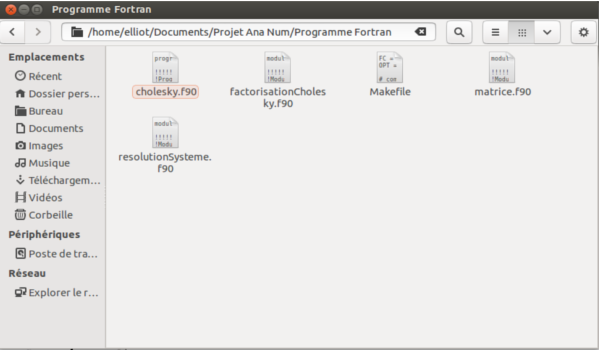
\includegraphics[scale = 0.5]{captureFichiers.png}
  				\caption{Les fichiers utilisés par notre programme}
		\end{figure}

		\begin{itemize}
			\item Le programme principal \textit{cholesky}, chef d'orchestre et fier de l'être
			\item Le module \textit{matrice} où sont regroupées deux procédures (ou subroutines) et une fonction : affichage de matrice carrée, de vecteur et étude de la symétrie de matrice carrée
			\item Le module \textit{factorisationCholesky}, qui, comme son nom l'indique, contient la procédure de factorisation de Cholesky sur une matrice carrée symétrique définie positive
			\item Le module \textit{resolutionSysteme} possédant deux procédures pour la remontée/descente et une procédure pour résoudre le système associé à une matrice carrée factorisée par la méthode de Cholesky  
			\item Et le fameux makefile pour nous simplifier la compilation.
		\end{itemize}

		Le code source commenté de tout ces fichiers se trouve en annexe.

		On remarquera notamment que l'écriture de l'algorithme de Cholesky s'en trouve grandement simplifiée en langage Fortran du fait des fonctions \textit{dot\_product} et \textit{matmul} permettant respectivement de multiplier les éléments des matrices entre eux ou d'effectuer un produit matriciel.
		On teste aussi, comme promis, si la factorisation fonctionne (on s'arrête à la moindre incohérence : division par $0$ ou bien passage à la racine d'un nombre négatif).


	\section{Précision machine}
		On prend un exemple tout bête :
			\[
				\begin{pmatrix}
					1 & -1 \\
					-1 & 4 \\
				\end{pmatrix}
				x =
				\begin{pmatrix}
					1 \\
					1 \\
				\end{pmatrix} \\
			\]
		La matrice est bien symétrique (évident) définie positive; en effet $\forall (x_{1}, x_{2}) \neq (0, 0)$ avec le produit scalaire canonique on a bien :
			\[
				\langle
				\begin{pmatrix}
					1 & -1 \\
					-1 & 4 \\
				\end{pmatrix}.
				\begin{pmatrix}
					x_{1} \\
					x_{2} \\
				\end{pmatrix},
				\begin{pmatrix}
					x_{1} \\
					x_{2} \\
				\end{pmatrix}
				\rangle \\ =
				\langle
				\begin{pmatrix}
					x_{1} - x_{2} \\
					-x_{1} + 4x_{2} \\
				\end{pmatrix},
				\begin{pmatrix}
					x_{1} \\
					x_{2} \\
				\end{pmatrix}
				\rangle \\ =
				x_{1}^{2} -x_{2}x_{1} -x_{1}x_{2} + 4x_{2}^{2} =
				(x_{1} - x_{2})^{2} + 3x_{2}^{2} > 0
			\]
		On trouve la solution du système linéaire en le résolvant à la main par la méthode de Gauss :
			\[
				\left\{
				\begin{array}{ll}
					x_{1} - x_{2} = 1 \\
					- x_{1} + 4x_{2} = 1 \\
				\end{array} \right. \\
				\Leftrightarrow
				\left\{
				\begin{array}{ll}
					x_{1} - x_{2} = 1 \\
					3x_{2} = 2 \\
				\end{array} \right. \\
			\]
		D'où :
			\[
				\left\{
				\begin{array}{ll}
					x_{1} = \frac{5}{3} \\
					x_{2} = \frac{2}{3} \\
				\end{array} \right. \\
			\]
		On lance le programme, qui est ici en précision simple ($real$, ou \og réels \fg{} sur $4$ octets) :
		\begin{figure}[!ht]
			\centering
  				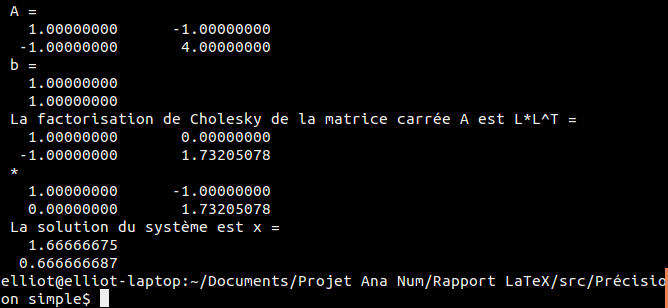
\includegraphics[scale = 0.5]{precisionsimple.png}
  				\caption{Le résultat du programme en précision simple}
		\end{figure}

		On devrait avoir :
		\[
			x = 
			\begin{pmatrix}
				1.66666666... \\
				0.66666666... \\
			\end{pmatrix}
		\]
		Or, à cause de la précision simple sur $4$ octets de la machine, on a malheureusement une erreur d'approximation à $10^{-6}$ près ici :
		\[
			x = 
			\begin{pmatrix}
				1.66666675 \\
				0.66666687 \\
			\end{pmatrix}
		\]

		Si l'on réitère l'opération en remplaçant tous les $real$ de notre programme Fortran par des $double$ $precision$ (\og réels \fg{} sur $8$ octets) on a :
		\begin{figure}[!ht]
			\centering
  				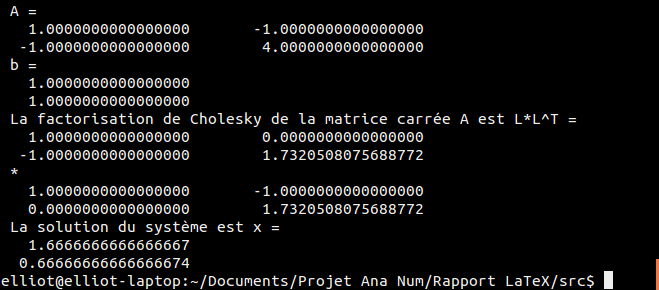
\includegraphics[scale = 0.5]{precisiondouble.png}
  				\caption{Le résultat du programme en précision double}
		\end{figure}
		\[
			x = 
			\begin{pmatrix}
				1.66666666666666667 \\
				0.66666666666666674 \\
			\end{pmatrix}
		\]

		Ici, l'erreur d'approximation se fait ressentir à $10^{-15}$ près sur la solution ce qui est bien meilleur ! Aujourd'hui, pour nos ordinateurs, $8$ octets en mémoire c'est très peu, autant profiter de cette précision supplémentaire.
		On fournira donc le programme en annexe avec des $double$ $precision$, libre au lecteur de modifier le code source à sa guise.

	
\chapter{Utilisation de la méthode pour résoudre des systèmes}
	\section{Premier système}
		On se propose de résoudre le système suivant :
			\[
				\begin{pmatrix}
					2 & -1 & 0 \\
					-1 & 2 & -1 \\
					0 & -1 & 2 \\
				\end{pmatrix}
				x =
				\begin{pmatrix}
					1 \\
					2 \\
					3 \\
				\end{pmatrix} \\
			\]
		Nous allons ici raisonner comme la machine, c'est-à-dire que nous commencerons par effectuer la factorisation de Cholesky pour pouvoir résoudre le système linéaire. En procédant de cette façon, on pourra vérifier les résultats donnés par notre programme pour la factorisation de Cholesky et la résolution du système.
		La matrice associée au système peut se décomposer de la manière suivante (en utilisant les formules du procédé de Cholesky) :
			\[
				\begin{pmatrix}
					2 & -1 & 0 \\
					-1 & 2 & -1 \\
					0 & -1 & 2 \\
				\end{pmatrix}
				=
				\begin{pmatrix}
					\sqrt{2} & 0 & 0 \\
					\frac{-1}{\sqrt{2}} & \sqrt{\frac{3}{2}} & 0 \\
					0 & -\sqrt{\frac{2}{3}} & \frac{2}{\sqrt{3}} \\
				\end{pmatrix} .
				\begin{pmatrix}
					\sqrt{2} & \frac{-1}{\sqrt{2}} & 0 \\
					0 & \sqrt{\frac{3}{2}} & -\sqrt{\frac{2}{3}}\\
					0 & 0 & \frac{2}{\sqrt{3}} \\
				\end{pmatrix}
			\]
		On résout ensuite le système suivant par descente :
			\[
				\begin{pmatrix}
					\sqrt{2} & 0 & 0 \\
					\frac{-1}{\sqrt{2}} & \sqrt{\frac{3}{2}} & 0 \\
					0 & -\sqrt{\frac{2}{3}} & \frac{2}{\sqrt{3}} \\
				\end{pmatrix}
				y =
				\begin{pmatrix}
					1 \\
					2 \\
					3 \\
				\end{pmatrix} \\
			\]
		Ce qui nous donne :
			\[
				y =
				\begin{pmatrix}
					\frac{1}{\sqrt{2}} \\
					\sqrt{\frac{3}{2}} \\
					\sqrt{3} \\
				\end{pmatrix} \\
			\]
		Il convient ensuite de résoudre par remontée :
			\[
				\begin{pmatrix}
					\sqrt{2} & \frac{-1}{\sqrt{2}} & 0 \\
					0 & \sqrt{\frac{3}{2}} & -\sqrt{\frac{2}{3}}\\
					0 & 0 & \frac{2}{\sqrt{3}} \\
				\end{pmatrix}
				x =
				\begin{pmatrix}
					\frac{1}{\sqrt{2}} \\
					\sqrt{\frac{3}{2}} \\
					\sqrt{3} \\
				\end{pmatrix} \\
			\]
		D'où :
			\[
				x =
				\begin{pmatrix}
					\frac{3}{2} \\
					2 \\
					\frac{3}{2} \\
				\end{pmatrix} \\
			\]
		\newpage
		Vérifions les résultats précédents avec notre programme :

		\begin{figure}[!ht]
			\centering
  				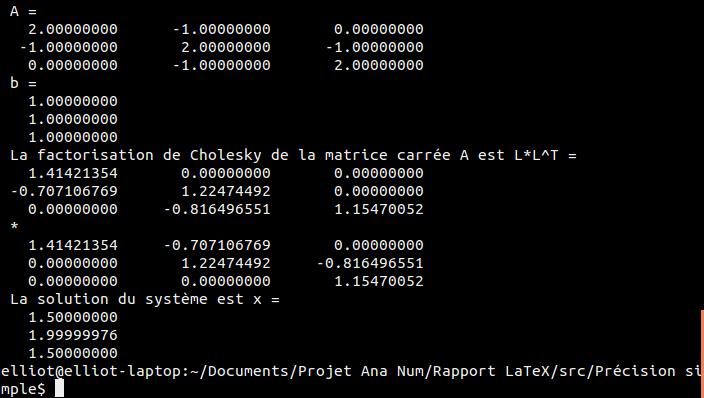
\includegraphics[scale = 0.4]{mat1simple.png}
  				\caption{Le résultat du programme sur le premier système en précision simple}
		\end{figure}

		\begin{figure}[!ht]
			\centering
  				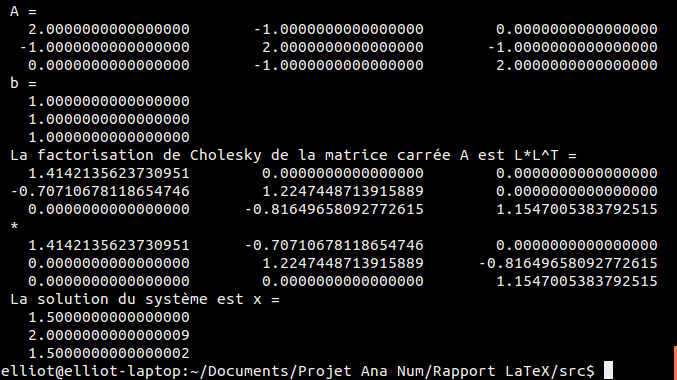
\includegraphics[scale = 0.4]{mat1double.png}
  				\caption{Le résultat du programme sur le premier système en double précision}
		\end{figure}
		Ces résultats coïncident avec les notres mais aussi avec ceux de MatLab (attention, la matrice de Cholesky retournée par la factorisation est ici celle triangulaire supérieure) :

		\begin{figure}[!ht]
			\centering
  				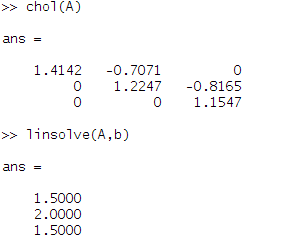
\includegraphics[scale = 0.4]{matlab1.png}
  				\caption{La même décomposition et la même résolution sur MatLab}
		\end{figure}
		\newpage
		On remarque toujours une approximation à $10^{-15}$ près en $double$ $precision$ et à $10^{-6}$ près en $real$. Cette même approximation se fait aussi ressentir sur le résultat de la décompositon de Cholesky.
		Cette précision est satisfaisante, cela peut s'expliquer par le conditionnement plutôt bon de la matrice (on rappelle que $\forall A \in \mathcal{M}_{n,n}, \ cond(A) \geq 1$) :

		\begin{figure}[!ht]
			\centering
  				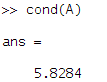
\includegraphics[scale = 0.6]{cond1.png}
  				\caption{Conditionnement de la matrice}
		\end{figure}
		En $real$, cela nous donne par exemple : $2 \approx 1,99999967$ ce qui porte à confusion.
		En effet, en $double$ $precision$ on a : $2 \approx 2,0000000000000009$ ce qui est plus précis et plus clair.

	\section{Second système}
		Nous allons ici essayer de résoudre ce système linéaire :
			\[
				\begin{pmatrix}
					10 & 7 & 8 & 7 \\
					7 & 5 & 6 & 5 \\
					8 & 6 & 10 & 9 \\
					7 & 5 & 9 & 10 \\
				\end{pmatrix}
				x =
				\begin{pmatrix}
					32 \\
					23 \\
					33 \\
					31 \\
				\end{pmatrix} \\
			\]
		Alors la décompostion de Cholesky nous donne :
			\[
				    \begin{pmatrix}
                        10 & 7 & 8 & 7\\
                        7 & 5 & 6 & 5\\
                        8 & 6 & 10 & 9\\
                        7 & 5 & 9 & 10\\
                    \end{pmatrix} =
                    \begin{pmatrix}
                        \sqrt{10} & 0 & 0 & 0\\
                         \frac{7}{\sqrt{{10}}} & \sqrt{\frac{1}{10}} & 0 & 0\\
                        \frac{8}{\sqrt{10}} & \frac{2}{5\sqrt{\frac{1}{10}}} & \sqrt{2} & 0\\
                        \frac{7}{\sqrt{10}} & \frac{1}{10}{\sqrt{\frac{1}{10}}} & \frac{3}{\sqrt{2}} & \sqrt{\frac{1}{2}}\\
                    \end{pmatrix}
                    \begin{pmatrix}
                        \sqrt{10} & \frac{7}{\sqrt{10}} & \frac{8}{\sqrt{10}} & \frac{7}{\sqrt{10}}\\
                        0 & \sqrt{\frac{1}{10}} & \frac{2}{5\sqrt{\frac{1}{10}}} & \frac{1}{10}{\sqrt{\frac{1}{10}}}\\
                        0 & 0 & \sqrt{2} & \frac{3}{\sqrt{2}}\\
                        0 & 0 & 0 & \sqrt{\frac{1}{2}}\\
                    \end{pmatrix}
			\]
		Pour résoudre ce système on utilise la méthode de descente.
		La résolution nous donne :
			\[
                    y =
                    \begin{pmatrix}
                        \frac{32}{\sqrt{10}} \\
                        \frac{3\sqrt{10}}{5} \\
                        \frac{5}{\sqrt{2}} \\
                        \frac{1}{2\sqrt{2}} \\
                    \end{pmatrix}
			\]
		Finalement pour trouver $x$ on applique la méthode de remontée et on a le résultat suivant :
			\[
                    x =
                    \begin{pmatrix}
                        1\\
                        1\\
                        1\\
                        1\\
                    \end{pmatrix}
			\]
		\newpage
		On vérifie alors les résultats précédents avec notre programme :

		\begin{figure}[!ht]
			\centering
  				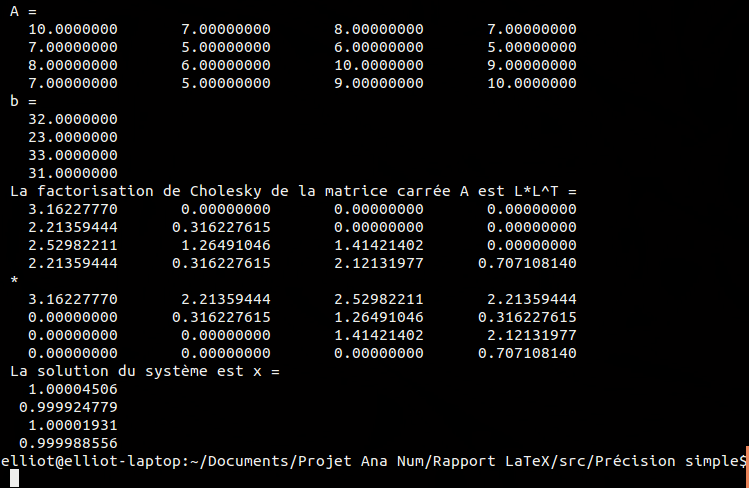
\includegraphics[scale = 0.4]{mat2simple.png}
  				\caption{Le résultat du programme sur le second système en précision simple}
		\end{figure}

		\begin{figure}[!ht]
			\centering
  				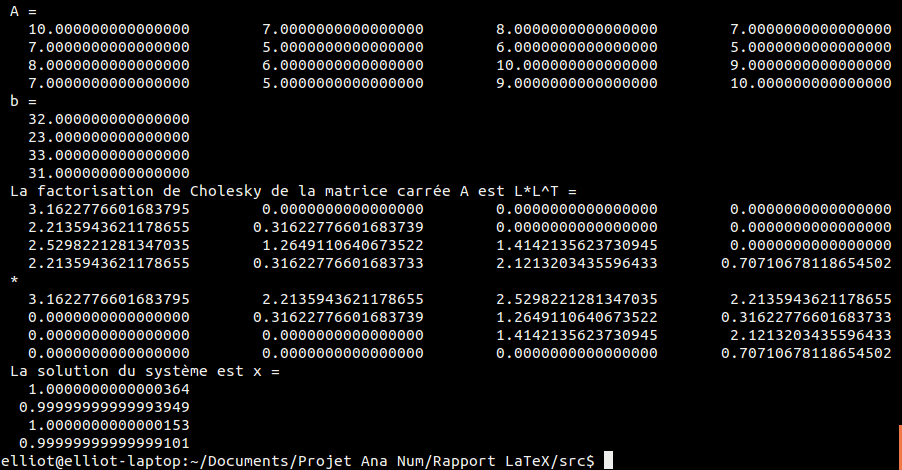
\includegraphics[scale = 0.4]{mat2double.png}
  				\caption{Le résultat du programme sur le second système en double précision}
		\end{figure}
		\newpage
		Là encore, ces résultats correspondent aux valeurs attendues sur papier et sur MatLab :

		\begin{figure}[!ht]
			\centering
  				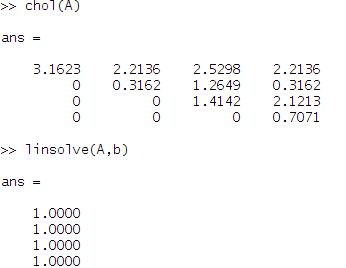
\includegraphics[scale = 0.4]{matlab2.png}
  				\caption{La même décomposition et la même résolution sur MatLab}
		\end{figure}
		Toutefois, la précision est de $10^{-4}$ en $real$ et $10^{-13}$ en $double$ $precision$.
		Le nombre de calculs effectués étant plus grand, on peut comprendre que cette approximation soit plus grossière.
		De plus, le conditionnement de la matrice est largement supérieur au précédent, cela explique en grande partie la raison de ce manque de précision ! L'approximation de la machine se fait bien plus ressentir sur le résultat.

		\begin{figure}[!ht]
			\centering
  				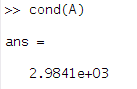
\includegraphics[scale = 0.6]{cond2.png}
  				\caption{Conditionnement de la matrice}
		\end{figure}

	\section{Petit bilan}
		Concernant la méthode de Cholesky, en effectuant sur MatLab le procédé de factorisation de Gauss et celui de Cholesky, on remarque une différence significative de rapidité d'exécution.
		Cela nous amène donc à la conclusion que, même si les critères d'applications sont plus restrictifs, il est préférable d'appliquer (lorsque c'est possible) Cholesky.

		De plus, nous avons ici remarqué numériquement que le conditionnement de la matrice associée à un système linéaire joue un rôle majeur (si ce n'est primordial) dans le calcul du vecteur résultant.
		Ainsi cet outil se révèlera indispensable à tout numéricien.
		Le calcul du condtionnement n'étant pas des plus évident, le \og magicien des nombres \fg{} s'enquerra surtout de son ordre de grandeur.
		Il en déduira ainsi, pour chaque coordonée de la solution, un intervalle dans lequel elle se situe.
		Savoir que l'on commet une erreur est une chose respectable, en connaître l'ampleur est d'autant plus sage.
		

\chapter*{Conclusion}
\addcontentsline{toc}{chapter}{Conclusion}													% ajouter la conclusion au sommaire
	Ce projet, d'une durée relativement limitée, nous aura néanmoins enseigné de nombreuses choses :
	\begin{itemize}
		\item Une connaissance accrue du contexte historique d'apparition de la méthode de Cholesky, incluant les méthodes antérieures à ce procédé
		\item Une meilleure compréhension de la méthode de factorisation $LL^{T}$ et de ses applications, notamment pour la résolution de systèmes linéaires
		\item Une maîtrise plus poussée du langage Fortran, et particulièremment de la norme $90$
		\item Une vision plus globale de la matière d'Analyse Numérique (GM3) que nous continuerons d'étudier toute l'année.
	\end{itemize}
	L'algorithme de Cholesky nous a ici permis de mettre en évidence des erreurs du à des \og perturbations \fg{} (dans nos exemples causées par la machine), accentuant ainsi le fait que la résolution d'un système ne repose pas uniquement sur la méthode d'approche de celui-ci.
	Le résultat n'a d'interêt que lorsqu'il est correctement approché. 
	Optimiser les calculs et limiter les approximations pour connaître au mieux la solution d'un problème donné, telle est la quête du numéricien.

\appendix

\chapter{Programme Fortran}
	\lstset{language=[90]Fortran,
		inputencoding=utf8/latin1
		}

	\section{Programme principal}
		Fichier : cholesky.f90

		\lstinputlisting{src/cholesky.f90}

	\section{Le module matrice}
		Fichier : matrice.f90
	
		\lstinputlisting{src/matrice.f90}

	\section{Le module factorisationCholesky}
		Fichier : factorisationCholesky.f90
	
		\lstinputlisting{src/factorisationCholesky.f90}

	\section{Le module resolutionSysteme}
		Fichier : resolutionSysteme.f90
	
		\lstinputlisting{src/resolutionSysteme.f90}

	\section{Le makefile}
		Fichier : makefile
		\lstset{language=make} 
	
		\lstinputlisting{src/Makefile}

\begin{thebibliography}{9}
\addcontentsline{toc}{chapter}{Bibliographie}													% permet de l'avoir dans le sommaire

	\bibitem{Cours 01}
		\emph{Anastasia Zakharova},
		\textit{Cours d'analyse numérique},
		Institut National des Sciences Appliquées de Rouen.

	\bibitem{Cours 02}
		\emph{Guillaume Legendre},
		\textit{Introduction à l'analyse numérique et au calcul scientifique},
		Dauphine, Paris.

	\bibitem{Cours 03}
		\emph{Pierre-Emmanuel Jabin},
		\textit{Corrigé d'analyse numérique, TD6},
		Université de Nice Sophia-Antipolis.

	\bibitem{Cours 04}
		\emph{Jocelyne Erhel, Nabil Nassif, Bernard Philippe},
		\textit{Calcul matriciel et systèmes linéaires},
		Institut National des Sciences Appliquées de Rennes.

	\bibitem{Cours 05}
		\emph{Jean-Guy Caputo},
		\textit{Cours de Fortran 77-90},
		Institut National des Sciences Appliquées de Rouen.

	\bibitem{Article 01}
		\emph{Claude Brezinski},
		\textit{Revue historique sur la méthode de Cholesky},
		Société mathématique de France, 2005.

	\bibitem{Lien Internet 01}
		\url{https://gist.github.com/pozdneev/866702}
		(Valide à la date du 20/10/2013)
		Une implémentation du procédé de Cholesky en Fortran 90/95 sans pivotage.

	\bibitem{Lien Internet 02}
		\url{https://github.com/bhermanmit/Fortran/blob/master/Lecture_4/examples/cholesky.f90}
		(Valide à la date du 20/10/2013)
		Une implémentation de la méthode de Cholesky en Fortran 90.

	\bibitem{Lien Internet 03}
		\url{ftp://ftp.numerical.rl.ac.uk/pub/jkr/toms/algorithm.pdf}
		(Valide à la date du 20/10/2013)
		Une autre implémentation de la méthode de Cholesky en Fortran 90.

	\bibitem{Lien Internet 04}
		\url{http://jean-pierre.moreau.pagesperso-orange.fr/Fortran/choles_f90.txt}
		(Valide à la date du 20/10/2013)
		Une dernière implémentation du procédé de Cholesky en Fortran 90, avec implémentation du calcul d'inverse de matrice, résolution de systèmes linéaires et calcul de détérminant.
	


\end{thebibliography}


\end{document}